\section{Exploring \dgs{} Bandwidth-Quality Trade-offs}\label{sec:bandw-adapt}

Post-training compression can help encode \dgs{} videos at different bit-rates for on-demand streaming.
%
Quantizing \dgs{} frames aggressively or reducing the octree depth can help produce frames whose compressed sizes match the target rate.
%
However, these techniques can compromise visual quality; ideally, one would like to find quantization parameters and resolutions that maximize quality for the target bitrate.
%
The best parameter choices are also content-dependent.

\parab{Rate-distortion curves.}
%
In video coding, practitioners~\cite{netflix_rdo} determine rate-distortion curves that capture the tradeoff between quality and bitrate.
%
The red line in \cref{fig:rate-dist-example} depicts such a curve, in which the x-axis is the rate, the y-axis is the quality (in PSNR), and each point on the red curve corresponds to the set of parameters that gives the highest quality at that rate.

For \dgs{}, we can obtain such a curve by searching the space of parameters.
%
For each possible parameter search, we can encode and decode a \gs{} frame from the video, compute the compressed size and quality, then compute the \textit{convex hull} of those size/quality pairs.
%
In \cref{fig:rate-dist-example}, the blue points represent the size/quality pairs, and the red curve the convex hull.
%
To encode a video at a rate $B$, we can simply use the parameters of the nearest point on the convex hull corresponding to rate $B$.
%
By the definition of the convex hull, this gives the highest quality, assuming we cover the search space well.

Two problems have prevented prior research in \dgs{} (\textit{e.g.}, \cite{gpcc-adaptive,queen}) from efficiently searching the parameter space.
%
First, their encode and decode latencies can be extremely high.
%
Second, the parameter space for \dgs{} is much larger than for 2-D video, since \gs{} frames can have 56 attributes, not including position.
%
Most prior work on post-compression training (\textit{e.g.}, \cite{mesongs}) applies \textit{selective quantization}, using different levels for different attributes.
%
That is because different attributes affect quality differently.
%
At one end, quantizing position attributes can introduce severe distortions because humans are very sensitive to geometry distortions.
%
At the other, quantizing SH coefficients aggressively only minimally impacts quality, since humans are less sensitive to color distortions, but also gives the biggest gains since, in many \gs{} frames, SH coefficients account for 70-80\% of the size.
%
To efficiently navigate this search space, some recent work~\cite{mga} has explored model-driven gradient ascent to guide the parameter search.

\gsnfs{}'s encoding and decoding speed addresses the first problem.
%
For example, \cref{fig:rate-dist-example} depicts the results of searching over a 1000 different parameter combinations using \gsnfs{}.
%
\ao{I understand that this means it is fast, but we haven't provided any context for how long it would take for other methods. }
This search takes about 12 minutes.

\begin{figure}[t]
  \centering
  \begin{tikzpicture}
    \node (R) {\includegraphics[width=0.7in]{figures/rgb_heatmap}};
    \node[below=0mm of R] (K) {\includegraphics[width=0.7in]{figures/klt_heatmap}};
    \node[fit=(R)(K)] (box) {};
    \node[left=0mm of box] (A) {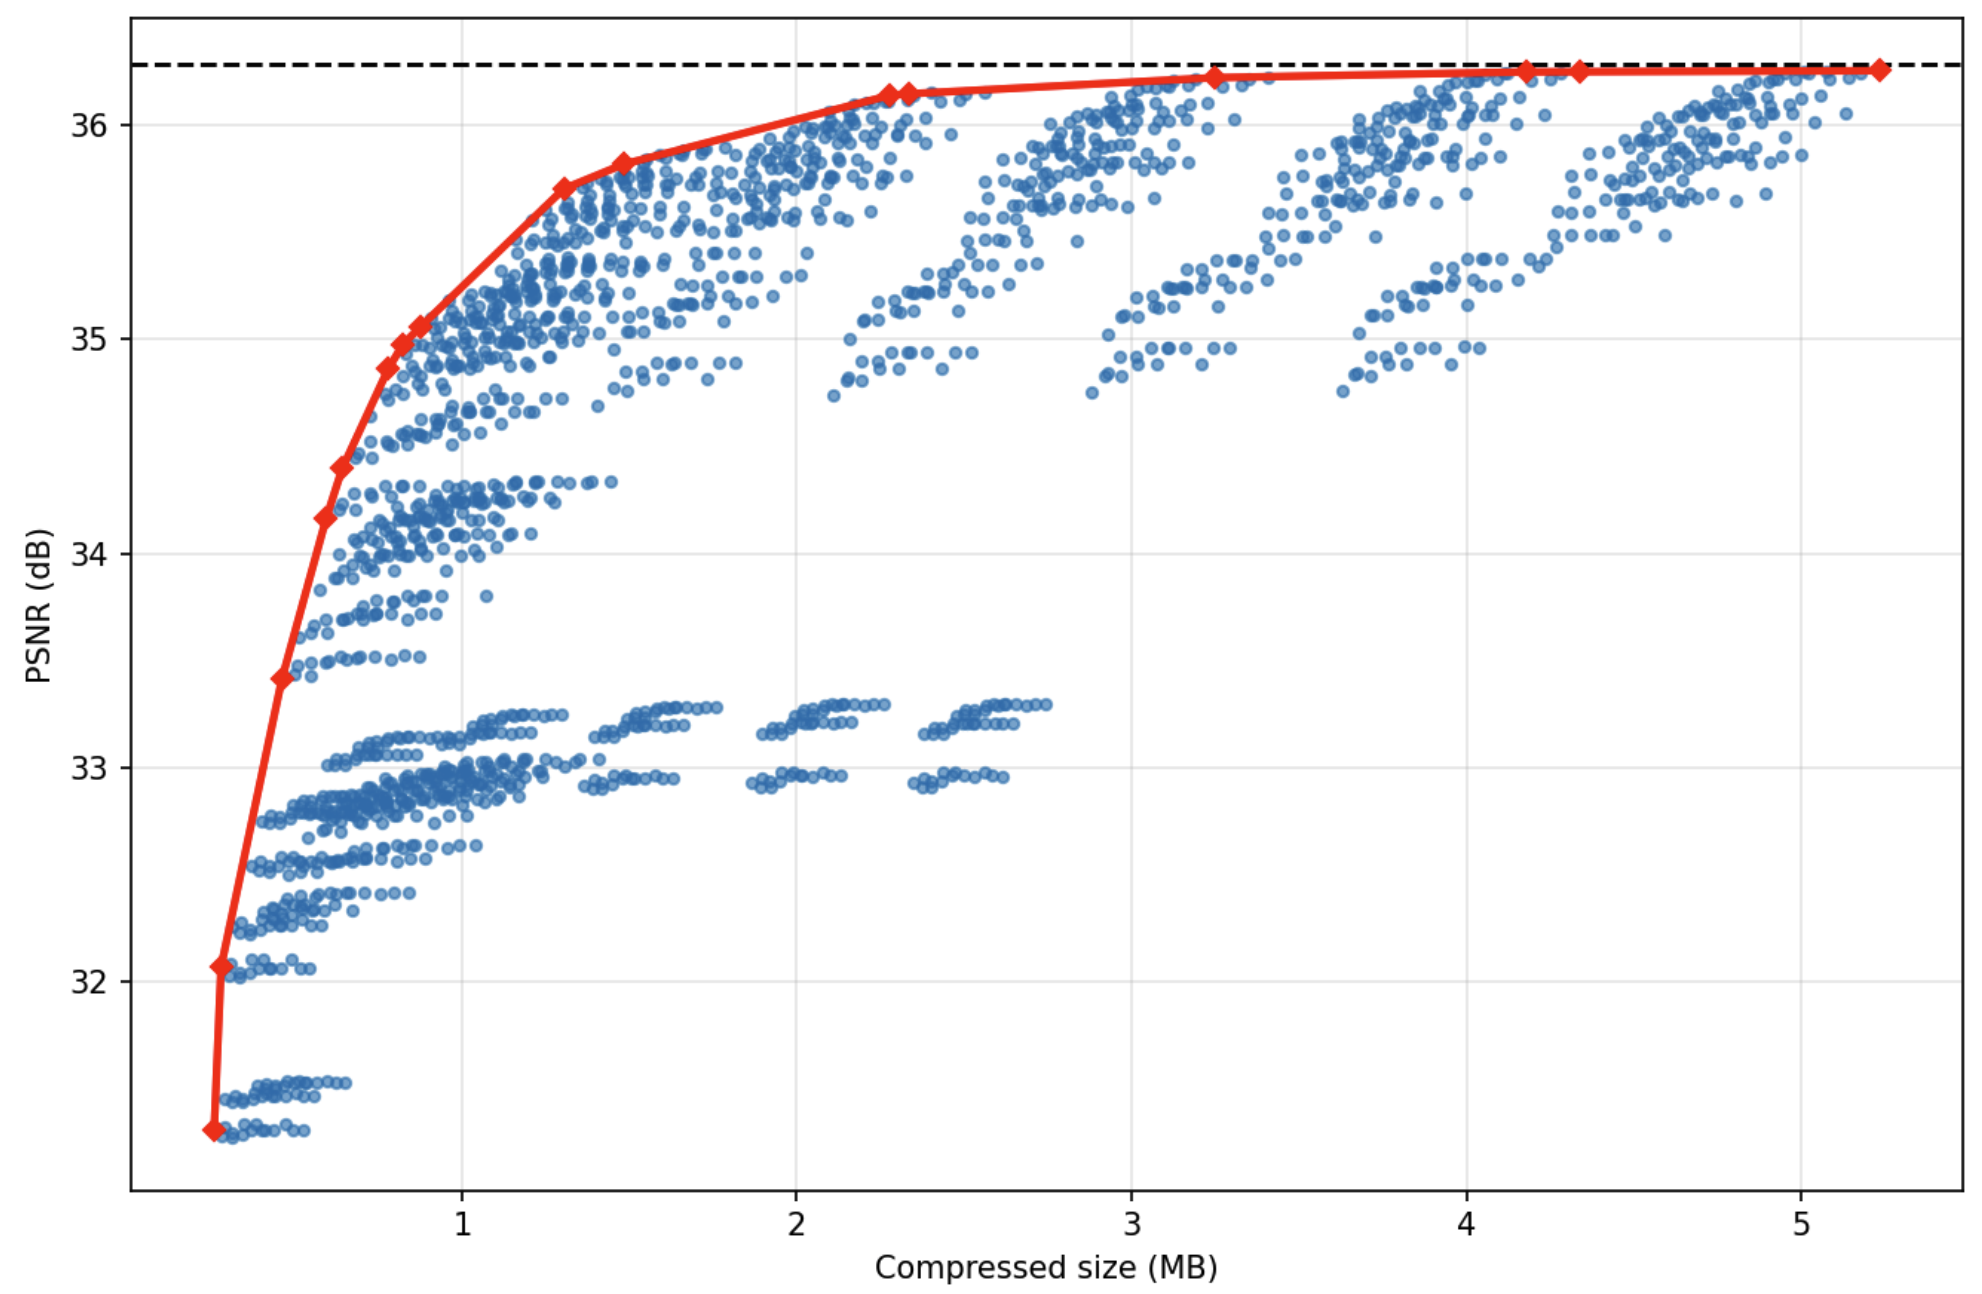
\includegraphics[width=2.2in]{figures/rate-dist-example.png}};
  \end{tikzpicture}  
  \caption{\label{fig:rate-dist-example} On the left is a rate-distortion plot, in which each point corresponds to a different parameter combination. Combinations on the convex hull produce the best quality at a given rate. On the right are two heatmaps that plot Pearson correlation across SHs before KLT (above) and after KLT (below).}
\end{figure}

\parab{Reducing search space using color de-correlation.}
%
We now describe an approach to address the second problem.
%
For \dgs{}, the search space is large in part because of the dimensionality of the SH coefficients---there are 48---which increases the search space dramatically.
%
As \cref{sec:3d-gauss-splatt} explains, these encode view-dependent color as coefficients of spherical harmonic functions of degree up to 3, and naïvely searching for quantization levels across all SH coefficients can be prohibitively expensive.

Now, it is well known that color across RGB channels can be correlated \cite{1990RGBcorr}. \ao{A reference?}\haoran{added}
%
In \gs{}, each degree of SH function has 3 coefficients in RGB space, and color correlations induce correlations both within SH coefficients of a single function, and across functions.
%
\gsnfs{} exploits this observation, and de-correlates these by first transforming the RGB to YUV for each degree of SH coefficients, then applying a de-correlating transform, the Karhunen-Loève transform (KLT~\cite{KLT}), to all AC SH coefficients within each YUV channel.
%
\eduardo{We are doing KLT only across degree 1,2,3 coeffs, except degree 0.}
\haoran{corrected to AC SH coeffs}
This decorrelation effectively concentrates signal energy on the first few coefficients.
%
\cref{fig:rate-dist-example} illustrates this.
%
On the top right is a heatmap of the Pearson correlation coefficients for the original RGB SH coefficients.
%
Below that is the corresponding heatmap after applying KLT; notice how the lower figure has significant white-space (white corresponds to zero correlation).
%
\ao{the main reason to use a decorrelating transform is that it arranges the outputs in order of decreasing average energy. For example, after taking the DCT of an 8x8 pixel block the frequencies (with a zig zag scan) can be ordered from highest to lowest energy and can be encoded in that order, so that the values after quantization are very likely to be zero (easier to encode). In our case that means that each successive RAHT transform with of a set of coefficients across Gaussians will have decreasing energy. We could use this to drop some of the lower RAHT coefficients completely (very likely they are all zero). It may also be possible to avoid using RAHT altogether for some KLT coefficients, because their spatial correlation may be too low. }
As a result of this, it suffices to \textit{use a single quantization parameter for 45 transform AC coefficients}, greatly reducing the search space.
%
\ao{In short, my point is that we do not need the KLT to use the same quantization parameter. We could have done this for the SH directly. }
KLT requires a matrix multiplication, which we implement on the GPU with minimal overhead.
%
An important benefit of KLT is increased compressibility, since it removes redundant information across SH channels.

%% \begin{comment}


%% \gsnfs uses a near-standard compression pipeline to produce a bit-stream by compressing both geomerty and attributes of \gs frames. 
%% %
%% Now, its design and careful implementation enables two practical optimizations for bitrate--quality tradeoffs that, to our knowledge, haven't been explored in prior \emph{post-training} \gs{} compression.
%% %
%% First, \gs{} appearance is encoded as DC (SH0) and AC coefficients (SH of order $> 0$), but these SH coefficients are correlated across RGB channels and across SH higher orders~\cref{fig:correlation-matrix}. 
%% %
%% This means they share redundant information forcing the entropy coder to waste bits if coded independently.
%% %
%% Decorrelating these coefficients will allow entropy coding spend fewer bits without hurting quality.
%% %
%% Second, quantization is the dominant source of information loss in a transform codec.
%% %
%% Different \gs{} attributes exhibit different sensitivity to quantization, and the best quantization settings depend on the content.
%% %
%% Because \gsnfs{} can perform fast encode/decode on GPU, we can efficiently search for per-video rate--distortion (R--D) operating points which enables superior bandwidth adaptation.

%% \subsection{SH coefficient channel and degree De-correlation}\label{sec:color-de-correlation}
%% Since RGB SH coefficients have high dimensions, independently coding coefficients in each dimension can consume more bits because it ignores the cross-channel and cross-degree correlation \cite{Liao2026}, leading to poor compression efficiency.

%% % channel
%% It is well-known that RGB color exhibits high cross-channel correlations. The same phenomenon is observed among RGB SH coefficients.
%% 3DGS can have infinite RGB values based on viewing angles. The RGB channels of the DC and AC SH coefficients of the splats are nearly perfectly correlated, likely due to the dominance of luminance over chrominance changes. This significant correlation suggests the feasibility of jointly encoding color across channels. 

%% To exploit this redundancy, we convert the RGB SH coefficients to the YUV color space. This transformation separates luminance from chrominance components, reducing channel redundancy and improving transform efficiency by concentrating most of the RGB energy in the Y (luminance) channel. Beyond compression gains, the conversion is also better aligned with human visual perception, which is more sensitive to brightness than to color differences. Consequently, we benefit from the YUV representation, which removes redundancy among the RGB channels and preserves perceptually important information in a single Y channel better aligned with human vision sensitivity.

%% % degree
%% Apart from cross-channel correlation, cross-degree correlation are also observed among SH coefficients. In 3DGS, YUV color typically varies smoothly with viewing direction. In real scenes, view-dependent color is often dominated by smooth specular lobes. Such smooth functions on the sphere requires SH spectral energy distributed across the degree like in the Fourier domain, rather than being concentrated at a single degree. For example, when approximating a specular lobe, low-degree SH bases capture its coarse directional structure, while higher-degree bases progressively refine and sharpen it. If the l=1 coefficients are large, the l=2 and l=3 coefficients are typically also predictably large. This is because bases across different degrees are jointly approximating the same smooth lobe, often aligned in similar directions and with related magnitudes.
%% As a result, the SH coefficients possess cross-degree correlation.

%% To remove SH cross-degree correlation, we compute the covariance of SH AC coefficients within each YUV channel to generate the eigenvectors sorted in increasing order of their associated eigenvalues. The eigenvectors are used to transform SH AC, known as the Karhunen-Loève transform (KLT). By applying KLT to SH AC within each YUV, the original energy distributed across the SH spectrum is fully decorrelated and mostly compacted into the first few KLT bases. The energy distribution over the KLT bases decays rapidly as the eigenvalues decrease, which favors the compression. 

%% Since 3DGS typically requires fewer than three degrees of SH representation, the computation of KLT bases is highly efficient. The computational complexity can be further reduced by allowing each Group of Frames to reuse the KLT bases computed from its first frame. Since the KLT bases are data-driven, they must be transmitted to the decoder as overhead information along with the compressed data. Decoding, therefore, requires both the KLT bases and the transform coefficients.



%% \begin{outline}

%%   Background
%%   \begin{itemize}
%%   \item Color correlation: correlation across RGB and why YUV de-correlates; when doing YUV, most important information is in Y. 
%%   \item Advantages: 
%%     \begin{itemize}
%%     \item There is lot of redundancy which wastes bits in entropy coding per channel. 
%%     \item The QP search space for SH is large when channels are correlated. We can search over few $\Delta_{AC}$, since energy is compacted in the first few ACs after KLT.
%%     \end{itemize}
%%   \item SH background: there is correlation across different harmonics
%%   \end{itemize}

%%   Key idea: de-correlate across Y channels; what do we do for U and V?

%%   Approach:
%%   \begin{itemize}
%%   \item Use KLT transform: simplify this perhaps with reference to PCA
%%   \item This keeps most energy in the first few Y entries, resulting in a rapidly decaying function.
%%   \end{itemize}

%%   Can incorporate this into our pipeline without impacting performance:
%%   \begin{itemize}
%%   \item encode step: how to generate the matrix, how to compute the KLT
%%   \item what needs to be transmitted
%%   \item what happens upon decode
%%   \end{itemize}
  
%% \end{outline}

%% \subsection{Selective Quantization}\label{sec:adapt-quant}

%% \begin{outline}

%%   Background:
%%   \begin{itemize}
%%   \item Rate-distortion curves; how this is applied to 2D video
%%   \item How it is generated and how it is used for on-demand video; perhaps explain Netflix's per-video RDO
%%   \end{itemize}

%%   Different attributes have different sensitivity to quantization/information loss
%%   \begin{itemize}
%%   \item Preserve geometry: don't quantize depth
%%   \item Compress minimally rotation, scale, and opacity
%%     \begin{itemize}
%%     \item Rotation and scale impact geometry
%%     \item Rendering is sensitive to opacity
%%     \end{itemize}
%%   \item Rest of attributes are spherical harmonics which determine color
%%     \begin{itemize}
%%       \item Humans are less sensitive to color
%%       \item Spherical harmonics account for very large fraction of GS by volume
%%       \end{itemize}
%%   \end{itemize}

%%   Explain what others do:
%%   \begin{itemize}
%%   \item V3 does not do anything
%%   \item MesonGS does VQ on SH, does not compress position, minimally compresses opacity, compresses scales and rotation similarly, and compresses SH uniformly without de-correlation
%%   \end{itemize}

%%   We: can efficiently search the space of quantization parameters and octree depth because of pipeline:

%%   Describe the process:
%%   \begin{itemize}
%%   \item For each parameter choice, compute PSNR and rate
%%   \item Find convex hull: include a picture of an RD curve
%%   \end{itemize}

%%   Describe how we can use the R-D curve
%%   \begin{itemize}
%%   \item Table lookup for rate, for DASH streaming
%%   \item Need to do this for a few frames (where scenes change)
%%   \end{itemize}
  
%% \end{outline}

%% Adaptive bitrate (ABR) streaming relies on the fact that compression exposes a continuous trade-off between \emph{rate} (bitrate or file size) and \emph{distortion} (quality loss).
%% %
%% In 2D video, this trade-off is commonly summarized by a \emph{rate--distortion (R--D) curve}, obtained by encoding the same content under different encoder settings \eg resolution and quantization step-size, measuring the resulting bitrate and quality, and retaining only Pareto-optimal operating points~\cite{2d-rdo}.
%% %
%% At scale, on-demand video services like YouTube and Netflix pre-compute these R--D points offline and select an efficient encoding ladder by taking the convex hull across all candidate videos~\cite{rdo-convex-hull}.
%% %
%% In recent years, Netflix generates per-title R--D analysis for individual videos or group of similar videos \eg cartoon vs action movies to obtain custom bitrate ladders~\cite{netflix_rdo,rdo-per-title-pcs,rdo-per-title-dcc}.
%% %
%% The resulting ladder enables a simple runtime decision: given a bandwidth estimate, the client/server picks the highest-quality representation whose rate fits the bandwidth budget.

%% \parab{Different 3DGS attributes have different sensitivity to quantization.}
%% Rate--distortion optimization (RDO) is essential for \dgs because each frame carries a large, high-dimensional set of Gaussians, and streaming must continuously trade bitrate against perceptual quality under time-varying network capacity.
%% %
%% However, in a \gs frame, the perceptual impact of quantization varies sharply across gemoetry (position) and various attribute types:
%% \begin{itemize}
%%   \item \textbf{Position:}
%%   Small perturbations in 3DGS positions can create noticeable reprojection artifacts (\eg popping/flicker) because  Gaussians shift on the image plane.
%%   %
%%   In \gsnfs, geometry is already compactly represented by octree occupancy but we allow fine to caorse voxelization (same as changing octree depth $J$). 
%%   %
%%   Note that we do not quantizate positions before entropy coding using ANS. (\S\ref{sec:octree-encode-gpu}).

%%   \item \textbf{Rotation, Scale, Opacity:}
%%   Rotation and scale determine the covariance of each Gaussian and thus affect geometric extent and transformation; opacity directly affects alpha compositing and is perceptually sensitive.
%%   %
%%   Over-quantizing these parameters can cause visible geometry deformation and transparency artifacts, so \gsnfs need to explore relatively small step sizes for these attributes (\ref{sec:quantization}).

%%   \item \textbf{Color:}
%%   The remaining parameters are spherical-harmonic (SH) coefficients that control view-dependent color.
%%   %
%%   Two observations make them prime targets for bitrate reduction:
%%   %
%%   (i) human vision is generally less sensitive to small chromatic errors than to geometric distortion~\cite{geometry-sensitivity1, geometry-sensitivity2}, and
%%   (ii) SH coefficients account for a large fraction of the per-Gaussian data ($48$ dimensions for SH up to degree 3).
%% \end{itemize}

%% Existing 3DGS streaming/compression systems acknowledge attribute sensitivity, but use comparatively coarse heuristics.
%% %
%% \vthree~\cite{v3volumetric} stores Gaussians as 2D images and encodes using H.264 with a single quantization parameter (QP) control.
%% %
%% Similar to \gsnfs, MesonGS~\cite{mesongs} compresses position using an octree, applies RAHT and block quantization to most attributes, while using vector quantization for higher-degree SH coefficients before packing with LZ77.
%% %
%% It improves compression, but it significantly limits the parameter space (octree depth, block size, and quantization step size) to few hand picked values due to high encoding latency.

%% \parab{\gsnfs's opportunity: fast offline exploration.}
%% Unlike prior approaches that rely on fixed or a small set of hand-tuned presets, \gsnfs can efficiently \emph{search} over codec parameters because the entire pipeline is GPU-resident and fast (\S\ref{sec:fast-compression}).
%% %
%% We treat selective quantization as a content-driven optimization problem: choose a parameter vector
%% \[
%% \theta = \big(J,\ \Delta_{\text{rot}},\Delta_{\text{scale}},\Delta_{\text{opacity}},\Delta_{\text{DC}},\Delta_{\text{AC}}\big),
%% \]
%% where $J$ is the voxel/octree depth and $\Delta_{\cdot}$ are per-attribute quantization step sizes.
%% %
%% Each choice of $\theta$ produces one operating point on the R--D plane.

%% \parab{Constructing the R--D curve.}
%% For each candidate $\theta$ in a predefined grid (or a coarse-to-fine search), \gsnfs follows this procedure for R--D exploration:
%% (a) encodes the few candidate frames in avideo using the GPU codec,
%% (b) decodes it and renders a fixed set of test views,
%% (c) measures distortion (PSNR/SSIM) against the uncompressed \gs frames, and
%% (d) records the achieved size.
%% %
%% This is analogous to how today's streaming platforms~\cite{netflix_rdo,rdo-per-title-dcc,rdo-per-title-pcs} generate R--D points per-title by probing multiple encoding parameters and analyzing quality vs rate.
%% %
%% We then discard dominated points and keep the convex hull (Pareto frontier), following the same principle used by video encoding ladders~\cite{rdo-convex-hull}.

%% \begin{figure}[t]
%%   \centering
%%   \includegraphics[width=\columnwidth]{example-image-a}
%%   \caption{Sample R--D curve with convex hull.}
%%   \label{fig:rd-curve}
%% \end{figure}

%% \parab{Use R--D curve for ABR streaming.}
%% The convex-hull points form a small set of \emph{representations} (a \dgs bitrate ladder).
%% %
%% At runtime, the sender (or client in DASH-like control) performs a simple table lookup: given an available bitrate, select the highest-quality point on the hull whose rate fits the bandwidth budget (estimated from streaming statistics).
%% %
%% \raj{Ramesh: Reason to do RDO for few frames? Current datasets have fixed cameras and limited dynamics in the scene. Is this reasoning compelling?}
%% %
%% \gsnfs's fast codec provides flexibility for streaming platforms to perform per-title RDO at any granularity compared to slow \dgs encoders with presets and in-training compression~\cite{queen,xxx} approaches that require retraining for each parameter choice.

%% \end{comment}
